% rubber: module pdftex

%% bare_conf.tex
%% V1.3
%% 2007/01/11
%% by Michael Shell
%% See:
%% http://www.michaelshell.org/
%% for current contact information.
%%
%% This is a skeleton file demonstrating the use of IEEEtran.cls
%% (requires IEEEtran.cls version 1.7 or later) with an IEEE conference paper.
%%
%% Support sites:
%% http://www.michaelshell.org/tex/ieeetran/
%% http://www.ctan.org/tex-archive/macros/latex/contrib/IEEEtran/
%% and
%% http://www.ieee.org/

%%*************************************************************************
%% Legal Notice:
%% This code is offered as-is without any warranty either expressed or
%% implied; without even the implied warranty of MERCHANTABILITY or
%% FITNESS FOR A PARTICULAR PURPOSE! 
%% User assumes all risk.
%% In no event shall IEEE or any contributor to this code be liable for
%% any damages or losses, including, but not limited to, incidental,
%% consequential, or any other damages, resulting from the use or misuse
%% of any information contained here.
%%
%% All comments are the opinions of their respective authors and are not
%% necessarily endorsed by the IEEE.
%%
%% This work is distributed under the LaTeX Project Public License (LPPL)
%% ( http://www.latex-project.org/ ) version 1.3, and may be freely used,
%% distributed and modified. A copy of the LPPL, version 1.3, is included
%% in the base LaTeX documentation of all distributions of LaTeX released
%% 2003/12/01 or later.
%% Retain all contribution notices and credits.
%% ** Modified files should be clearly indicated as such, including  **
%% ** renaming them and changing author support contact information. **
%%
%% File list of work: IEEEtran.cls, IEEEtran_HOWTO.pdf, bare_adv.tex,
%%                    bare_conf.tex, bare_jrnl.tex, bare_jrnl_compsoc.tex
%%*************************************************************************

% *** Authors should verify (and, if needed, correct) their LaTeX system  ***
% *** with the testflow diagnostic prior to trusting their LaTeX platform ***
% *** with production work. IEEE's font choices can trigger bugs that do  ***
% *** not appear when using other class files.                            ***
% The testflow support page is at:
% http://www.michaelshell.org/tex/testflow/



% Note that the a4paper option is mainly intended so that authors in
% countries using A4 can easily print to A4 and see how their papers will
% look in print - the typesetting of the document will not typically be
% affected with changes in paper size (but the bottom and side margins will).
% Use the testflow package mentioned above to verify correct handling of
% both paper sizes by the user's LaTeX system.
%
% Also note that the "draftcls" or "draftclsnofoot", not "draft", option
% should be used if it is desired that the figures are to be displayed in
% draft mode.
%
\documentclass[conference]{IEEEtran}
% Add the compsoc option for Computer Society conferences.
%
% If IEEEtran.cls has not been installed into the LaTeX system files,
% manually specify the path to it like:
% \documentclass[conference]{../sty/IEEEtran}



\usepackage[sort&compress,square,numbers]{natbib}
% some common packages
\usepackage{xspace}
\usepackage{url}
\usepackage{verbatim}
\usepackage{graphicx}
\usepackage{caption}
\usepackage{subcaption}
%\usepackage{algorithm, algorithmicx}
\usepackage{algorithm}
\usepackage{algpseudocode}
\usepackage{amsmath}
\usepackage{listings}
\usepackage{url}
\usepackage{float}
% user-defined macros
%\input{macros}




% Some very useful LaTeX packages include:
% (uncomment the ones you want to load)


% *** MISC UTILITY PACKAGES ***
%
%\usepackage{ifpdf}
% Heiko Oberdiek's ifpdf.sty is very useful if you need conditional
% compilation based on whether the output is pdf or dvi.
% usage:
% \ifpdf
%   % pdf code
% \else
%   % dvi code
% \fi
% The latest version of ifpdf.sty can be obtained from:
% http://www.ctan.org/tex-archive/macros/latex/contrib/oberdiek/
% Also, note that IEEEtran.cls V1.7 and later provides a builtin
% \ifCLASSINFOpdf conditional that works the same way.
% When switching from latex to pdflatex and vice-versa, the compiler may
% have to be run twice to clear warning/error messages.






% *** CITATION PACKAGES ***
%
%\usepackage{cite}
% cite.sty was written by Donald Arseneau
% V1.6 and later of IEEEtran pre-defines the format of the cite.sty package
% \cite{} output to follow that of IEEE. Loading the cite package will
% result in citation numbers being automatically sorted and properly
% "compressed/ranged". e.g., [1], [9], [2], [7], [5], [6] without using
% cite.sty will become [1], [2], [5]--[7], [9] using cite.sty. cite.sty's
% \cite will automatically add leading space, if needed. Use cite.sty's
% noadjust option (cite.sty V3.8 and later) if you want to turn this off.
% cite.sty is already installed on most LaTeX systems. Be sure and use
% version 4.0 (2003-05-27) and later if using hyperref.sty. cite.sty does
% not currently provide for hyperlinked citations.
% The latest version can be obtained at:
% http://www.ctan.org/tex-archive/macros/latex/contrib/cite/
% The documentation is contained in the cite.sty file itself.






% *** GRAPHICS RELATED PACKAGES ***
%
\ifCLASSINFOpdf
  % \usepackage[pdftex]{graphicx}
  % declare the path(s) where your graphic files are
  % \graphicspath{{../pdf/}{../jpeg/}}
  % and their extensions so you won't have to specify these with
  % every instance of \includegraphics
  % \DeclareGraphicsExtensions{.pdf,.jpeg,.png}
\else
  % or other class option (dvipsone, dvipdf, if not using dvips). graphicx
  % will default to the driver specified in the system graphics.cfg if no
  % driver is specified.
  % \usepackage[dvips]{graphicx}
  % declare the path(s) where your graphic files are
  % \graphicspath{{../eps/}}
  % and their extensions so you won't have to specify these with
  % every instance of \includegraphics
  % \DeclareGraphicsExtensions{.eps}
\fi
% graphicx was written by David Carlisle and Sebastian Rahtz. It is
% required if you want graphics, photos, etc. graphicx.sty is already
% installed on most LaTeX systems. The latest version and documentation can
% be obtained at: 
% http://www.ctan.org/tex-archive/macros/latex/required/graphics/
% Another good source of documentation is "Using Imported Graphics in
% LaTeX2e" by Keith Reckdahl which can be found as epslatex.ps or
% epslatex.pdf at: http://www.ctan.org/tex-archive/info/
%
% latex, and pdflatex in dvi mode, support graphics in encapsulated
% postscript (.eps) format. pdflatex in pdf mode supports graphics
% in .pdf, .jpeg, .png and .mps (metapost) formats. Users should ensure
% that all non-photo figures use a vector format (.eps, .pdf, .mps) and
% not a bitmapped formats (.jpeg, .png). IEEE frowns on bitmapped formats
% which can result in "jaggedy"/blurry rendering of lines and letters as
% well as large increases in file sizes.
%
% You can find documentation about the pdfTeX application at:
% http://www.tug.org/applications/pdftex





% *** MATH PACKAGES ***
%
%\usepackage[cmex10]{amsmath}
% A popular package from the American Mathematical Society that provides
% many useful and powerful commands for dealing with mathematics. If using
% it, be sure to load this package with the cmex10 option to ensure that
% only type 1 fonts will utilized at all point sizes. Without this option,
% it is possible that some math symbols, particularly those within
% footnotes, will be rendered in bitmap form which will result in a
% document that can not be IEEE Xplore compliant!
%
% Also, note that the amsmath package sets \interdisplaylinepenalty to 10000
% thus preventing page breaks from occurring within multiline equations. Use:
%\interdisplaylinepenalty=2500
% after loading amsmath to restore such page breaks as IEEEtran.cls normally
% does. amsmath.sty is already installed on most LaTeX systems. The latest
% version and documentation can be obtained at:
% http://www.ctan.org/tex-archive/macros/latex/required/amslatex/math/





% *** SPECIALIZED LIST PACKAGES ***
%
%\usepackage{algorithmic}
% algorithmic.sty was written by Peter Williams and Rogerio Brito.
% This package provides an algorithmic environment fo describing algorithms.
% You can use the algorithmic environment in-text or within a figure
% environment to provide for a floating algorithm. Do NOT use the algorithm
% floating environment provided by algorithm.sty (by the same authors) or
% algorithm2e.sty (by Christophe Fiorio) as IEEE does not use dedicated
% algorithm float types and packages that provide these will not provide
% correct IEEE style captions. The latest version and documentation of
% algorithmic.sty can be obtained at:
% http://www.ctan.org/tex-archive/macros/latex/contrib/algorithms/
% There is also a support site at:
% http://algorithms.berlios.de/index.html
% Also of interest may be the (relatively newer and more customizable)
% algorithmicx.sty package by Szasz Janos:
% http://www.ctan.org/tex-archive/macros/latex/contrib/algorithmicx/




% *** ALIGNMENT PACKAGES ***
%
%\usepackage{array}
% Frank Mittelbach's and David Carlisle's array.sty patches and improves
% the standard LaTeX2e array and tabular environments to provide better
% appearance and additional user controls. As the default LaTeX2e table
% generation code is lacking to the point of almost being broken with
% respect to the quality of the end results, all users are strongly
% advised to use an enhanced (at the very least that provided by array.sty)
% set of table tools. array.sty is already installed on most systems. The
% latest version and documentation can be obtained at:
% http://www.ctan.org/tex-archive/macros/latex/required/tools/


%\usepackage{mdwmath}
%\usepackage{mdwtab}
% Also highly recommended is Mark Wooding's extremely powerful MDW tools,
% especially mdwmath.sty and mdwtab.sty which are used to format equations
% and tables, respectively. The MDWtools set is already installed on most
% LaTeX systems. The lastest version and documentation is available at:
% http://www.ctan.org/tex-archive/macros/latex/contrib/mdwtools/


% IEEEtran contains the IEEEeqnarray family of commands that can be used to
% generate multiline equations as well as matrices, tables, etc., of high
% quality.


%\usepackage{eqparbox}
% Also of notable interest is Scott Pakin's eqparbox package for creating
% (automatically sized) equal width boxes - aka "natural width parboxes".
% Available at:
% http://www.ctan.org/tex-archive/macros/latex/contrib/eqparbox/





% *** SUBFIGURE PACKAGES ***
%\usepackage[tight,footnotesize]{subfigure}
% subfigure.sty was written by Steven Douglas Cochran. This package makes it
% easy to put subfigures in your figures. e.g., "Figure 1a and 1b". For IEEE
% work, it is a good idea to load it with the tight package option to reduce
% the amount of white space around the subfigures. subfigure.sty is already
% installed on most LaTeX systems. The latest version and documentation can
% be obtained at:
% http://www.ctan.org/tex-archive/obsolete/macros/latex/contrib/subfigure/
% subfigure.sty has been superceeded by subfig.sty.



%\usepackage[caption=false]{caption}
%\usepackage[font=footnotesize]{subfig}
% subfig.sty, also written by Steven Douglas Cochran, is the modern
% replacement for subfigure.sty. However, subfig.sty requires and
% automatically loads Axel Sommerfeldt's caption.sty which will override
% IEEEtran.cls handling of captions and this will result in nonIEEE style
% figure/table captions. To prevent this problem, be sure and preload
% caption.sty with its "caption=false" package option. This is will preserve
% IEEEtran.cls handing of captions. Version 1.3 (2005/06/28) and later 
% (recommended due to many improvements over 1.2) of subfig.sty supports
% the caption=false option directly:
%\usepackage[caption=false,font=footnotesize]{subfig}
%
% The latest version and documentation can be obtained at:
% http://www.ctan.org/tex-archive/macros/latex/contrib/subfig/
% The latest version and documentation of caption.sty can be obtained at:
% http://www.ctan.org/tex-archive/macros/latex/contrib/caption/




% *** FLOAT PACKAGES ***
%
%\usepackage{fixltx2e}
% fixltx2e, the successor to the earlier fix2col.sty, was written by
% Frank Mittelbach and David Carlisle. This package corrects a few problems
% in the LaTeX2e kernel, the most notable of which is that in current
% LaTeX2e releases, the ordering of single and double column floats is not
% guaranteed to be preserved. Thus, an unpatched LaTeX2e can allow a
% single column figure to be placed prior to an earlier double column
% figure. The latest version and documentation can be found at:
% http://www.ctan.org/tex-archive/macros/latex/base/



%\usepackage{stfloats}
% stfloats.sty was written by Sigitas Tolusis. This package gives LaTeX2e
% the ability to do double column floats at the bottom of the page as well
% as the top. (e.g., "\begin{figure*}[!b]" is not normally possible in
% LaTeX2e). It also provides a command:
%\fnbelowfloat
% to enable the placement of footnotes below bottom floats (the standard
% LaTeX2e kernel puts them above bottom floats). This is an invasive package
% which rewrites many portions of the LaTeX2e float routines. It may not work
% with other packages that modify the LaTeX2e float routines. The latest
% version and documentation can be obtained at:
% http://www.ctan.org/tex-archive/macros/latex/contrib/sttools/
% Documentation is contained in the stfloats.sty comments as well as in the
% presfull.pdf file. Do not use the stfloats baselinefloat ability as IEEE
% does not allow \baselineskip to stretch. Authors submitting work to the
% IEEE should note that IEEE rarely uses double column equations and
% that authors should try to avoid such use. Do not be tempted to use the
% cuted.sty or midfloat.sty packages (also by Sigitas Tolusis) as IEEE does
% not format its papers in such ways.





% *** PDF, URL AND HYPERLINK PACKAGES ***
%
%\usepackage{url}
% url.sty was written by Donald Arseneau. It provides better support for
% handling and breaking URLs. url.sty is already installed on most LaTeX
% systems. The latest version can be obtained at:
% http://www.ctan.org/tex-archive/macros/latex/contrib/misc/
% Read the url.sty source comments for usage information. Basically,
% \url{my_url_here}.





% *** Do not adjust lengths that control margins, column widths, etc. ***
% *** Do not use packages that alter fonts (such as pslatex).         ***
% There should be no need to do such things with IEEEtran.cls V1.6 and later.
% (Unless specifically asked to do so by the journal or conference you plan
% to submit to, of course. )


% correct bad hyphenation here
\hyphenation{op-tical net-works semi-conduc-tor}


\begin{document}
%
% paper title
% can use linebreaks \\ within to get better formatting as desired
\title{Detecting Safe Transformation of Immutable Objects using Escape Analysis}


% author names and affiliations
% use a multiple column layout for up to three different
% affiliations
\author{\IEEEauthorblockN{%
Atulan Zaman
\IEEEauthorblockA{Electrical and Computer Engineering\\
University of Waterloo \\
\url{a3zaman@uwaterloo.ca}}
%\and
}% end IEEEauthorblockN
}% end author 

% conference papers do not typically use \thanks and this command
% is locked out in conference mode. If really needed, such as for
% the acknowledgment of grants, issue a \IEEEoverridecommandlockouts
% after \documentclass

% for over three affiliations, or if they all won't fit within the width
% of the page, use this alternative format:
% 
%\author{\IEEEauthorblockN{Michael Shell\IEEEauthorrefmark{1},
%Homer Simpson\IEEEauthorrefmark{2},
%James Kirk\IEEEauthorrefmark{3}, 
%Montgomery Scott\IEEEauthorrefmark{3} and
%Eldon Tyrell\IEEEauthorrefmark{4}}
%\IEEEauthorblockA{\IEEEauthorrefmark{1}School of Electrical and Computer Engineering\\
%Georgia Institute of Technology,
%Atlanta, Georgia 30332--0250\\ Email: see http://www.michaelshell.org/contact.html}
%\IEEEauthorblockA{\IEEEauthorrefmark{2}Twentieth Century Fox, Springfield, USA\\
%Email: homer@thesimpsons.com}
%\IEEEauthorblockA{\IEEEauthorrefmark{3}Starfleet Academy, San Francisco, California 96678-2391\\
%Telephone: (800) 555--1212, Fax: (888) 555--1212}
%\IEEEauthorblockA{\IEEEauthorrefmark{4}Tyrell Inc., 123 Replicant Street, Los Angeles, California 90210--4321}}




% use for special paper notices
%\IEEEspecialpapernotice{(Invited Paper)}




% make the title area
\maketitle
\pagestyle{headings}
\setcounter{page}{1}
\pagenumbering{arabic}

\begin{abstract}
Immutable objects are preferred in Object Oriented Programming because of their safety and simplicity. However declaring all objects and data structures as immutable often causes heavy performance overhead for software programs. This is especially true for compilers where the entire Abstract Syntax Tree has to be rebuilt everytime the tree needs to be mutated. Therefore the work of this project looks at using static analysis to detect cases where objects can be safely transformed to be mutable from being immutable without compromising functionality and security. The basis of the analysis is using \textit{Escape Analysis} to detect escaping objects using intra-procedural dataflow analysis and Object Representatives.
\end{abstract}

\tableofcontents

% IEEEtran.cls defaults to using nonbold math in the Abstract.
% This preserves the distinction between vectors and scalars. However,
% if the conference you are submitting to favors bold math in the abstract,
% then you can use LaTeX's standard command \boldmath at the very start
% of the abstract to achieve this. Many IEEE journals/conferences frown on
% math in the abstract anyway.

% no keywords
\section{Introduction}
%Goodness(Cite immutability sideeffects)
Object immutability is a feature of object oriented programming that restricts objects from being mutated after they are instantiated. This is generally a recommended practice because of simplicity and safety of programs to prevent bugs. Object immutability comes in different forms. One of the forms is variable immutability. In Java for example, this is enforced by declaring variables as \texttt{final} so that it can only be set during object construction and cannot be mutated afterwards using mutator method. Second form of immutability is reference immutability. This ensures that external methods referencing to a mutable parameter does not have permissions to mutate the parameter. There is much research aimed at enforcing this form immutability, most notably the work of Huang et.\ al \citep{ref:ReIm} in creating a type system to ensure reference immutability when the referenced object is stored in a local variable. The work of Tschantz et. al on the tool \textit{Javari} \cite{ref:javari} is another research tool that helps programmers enforce reference immutability. At the class level, an object can be declared to be mutable if two design choices are maintained. Firstly, all the attributes of the class are declared to be immutable during declaration. Secondly all the mutator methods of the class retain the immutable nature of the object by creating a different instance of the object with the mutated attribute and returning that object instead of directly mutating the instance. 

This is generally desirable because that causes methods sharing the object to not behave erroneously. Another application of this is in concurrent programming where threads sharing objects will have their own instances of the object. However, sometimes this causes overhead because everytime an object needs to be mutated, the a new instance has to be reconstructed from the existing instance. It is a standard safety vs performance tradeoff in software engineering. For large instance manipulation such as in manipulating abstract syntax tree construction in compilers this causes high memory and performance footprint during the construction process. Due to safety recommendations of object oriented programming, programmer usual choose to make object instances immutable to ensure safety of execution. However in cases of object sharing, infered using escape analysis \citep{ref:compositionalEscape}\cite{ref:escapejava}\cite{ref:incrementalescape} it is provable that program safety can be ensure without enforcing object immutability. The work of this project focuses on using intra-procedural escape analysis techniques \cite{ref:Kotzmann} to detect cases where it is safe make objects mutable without any side effects.

This techniques uses intra-procedural dataflow analysis using object representatives \citep{ref:or} detect locals and references that share a common heap pointer. Object representatives is a technique for detecting variables that share the same heap pointer, although they have different stack pointers, without doing inter-procedural analysis. After the object representative mapping is created using a may alias analysis, our escape analysis heuristics are used to analyze program points to detect locals and references that might have escaped. The intra-procedural analysis in this project is implemented using the Soot framework for Java bytecode analysis \citep{ref:Soot}.

Much of program analysis research has been focused on detecting lack of immutability in program to detect potential sources of bugs and problems. Some work has been done on creating type systems to detect variables that behave like immutable although they are not declared as \texttt{final}\cite{ref:finalinference}. This work in a way is going against the flow of traditional research in the sense that it tries to escape from the paranoia of safety by trying to make immutable objects immutable.

%Related works(Cite javari, ReimInfer etc)
%Where does it fit in
%Analysis used(Cite Escape Analysis)
%Implementation(Cite Soot)
%Flow of the document

\section{Example}\label{sec:example}
In this section a motivating example of this work is explained. First a class with an immutable object declaration is presented, where a case is shown when it is safe to transform the class to a mutable object. Following the positive example, a case is presented which explains when it is not possible to transform an immutable class to mutable. The point of the analysis is to recognize the cases when an object cannot be transformed to mutable due to the nature of its usage by the caller of the object.
%The Immutable class

\begin{figure}[H]
	\caption{Immutable Object} \label{fig:immutable_object}
	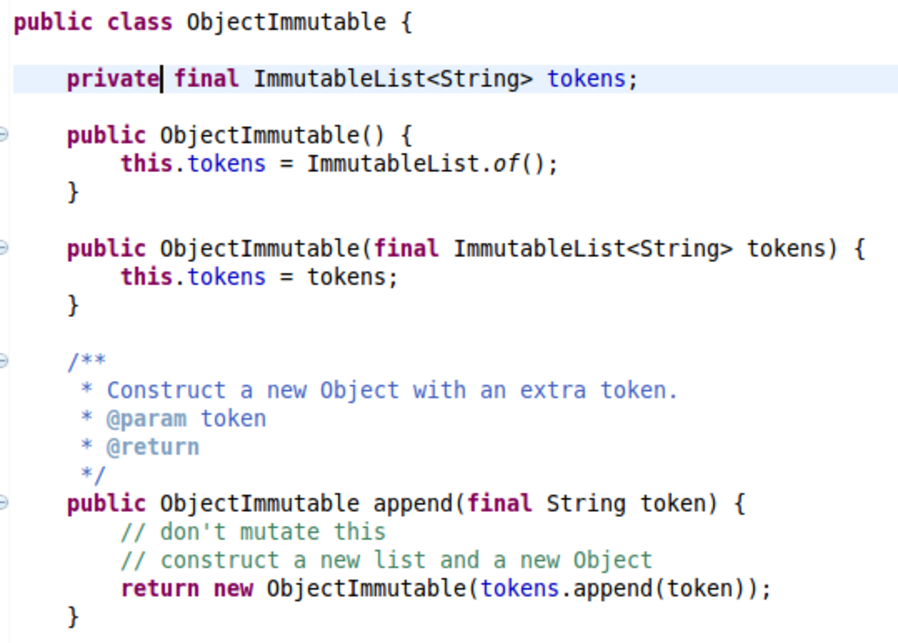
\includegraphics[width=0.5\textwidth]{img/immutable_object}
\end{figure}

\begin{figure}[H]
	\caption{Client without object escaping} \label{fig:clientNoEscape}
	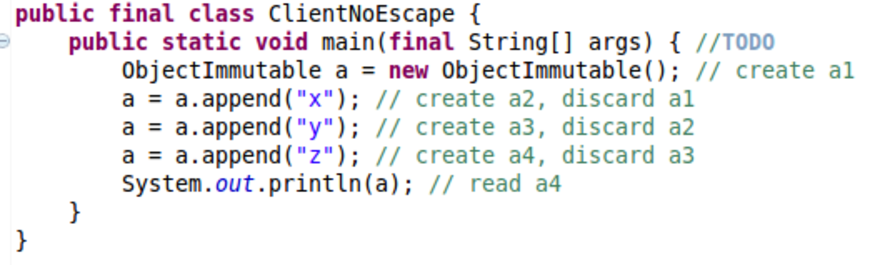
\includegraphics[width=0.5\textwidth]{img/client_noescape}
\end{figure}

In this example object shown in figure \ref{fig:immutable_object} it is evident that the object is immutable by the fact that the \texttt{token} attribute is \textit{final} and that the mutator method, \texttt{append\(\)} returns an instance of the mutated object rather than mutating the subject instance and returning a \texttt{void} type. Now let's look at figure \ref{fig:clientNoEscape} which shows the instance of a client object calling the immutable object. In this method all that is happening is that the client is appending to the initially created instance and finally it prints the most recent instance of the object to the console. In this case, since the initialized immutable object is not assigned to other globally accessible varible such as a \texttt{static} variable, or that it is not being passed as a parameter to another method, it is evident that within this caller, the object is not ``escaping''. The conditions for escape analysis that are used in this project are discussed later on in section \ref{sec:escape}.
Therefore if the this is the only client calling the the immutable object then it would be safe to transform the immutable object to an mutable object, because a reference of the object is not assigned to the heap before the end of execution of the method.

\begin{figure}[H]
	\caption{Transformed Mutable Object} \label{fig:mutableobj}
	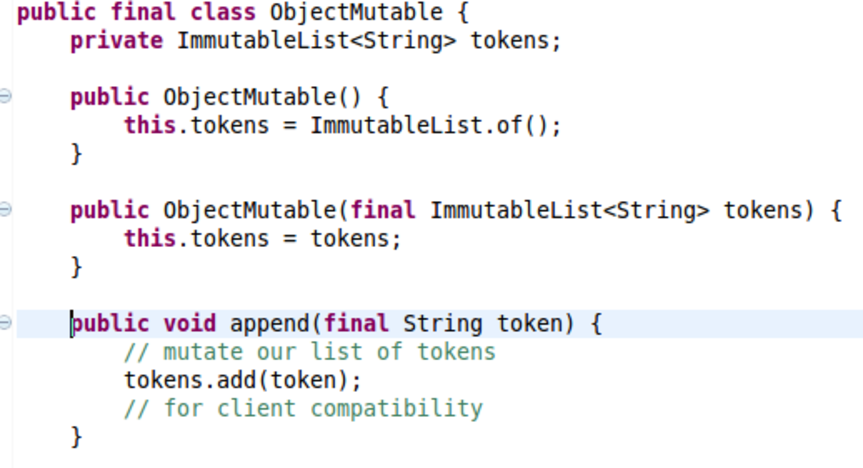
\includegraphics[width=0.5\textwidth]{img/mutable_object}
\end{figure}

\begin{figure}[H]
	\caption{Transformed Client Object} \label{fig:transformedclient}
	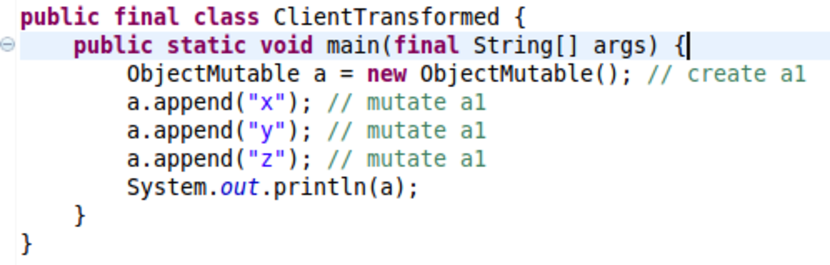
\includegraphics[width=0.5\textwidth]{img/client_transformed}
\end{figure}

A possible transformation of the immutable object can be viewed in figure \ref{fig:mutableobj}. In figure \ref{fig:mutableobj} it is evident that that only difference the immutable object and this are three transformations:
\begin{itemize}
\item The local variable has been changed from \texttt{private final} to just \texttt{private}.
\item The mutator method \texttt{append} has been changed to return a \texttt{void} type.
\item The mutator method directly appends to the \texttt{ImmutableList} attribute.
\end{itemize}

Because of the change in the object implementation. All the calling sites of the object also needs to be refactored in order to make this change effective. In figure \ref{fig:transformedclient} the transformed client is shown. The changes that happen to the client are at the program points where the client calls the mutator method of the transformed mutable object.

\begin{figure}[H]
	\caption{Client with Escaping Object} \label{fig:client_escape}
	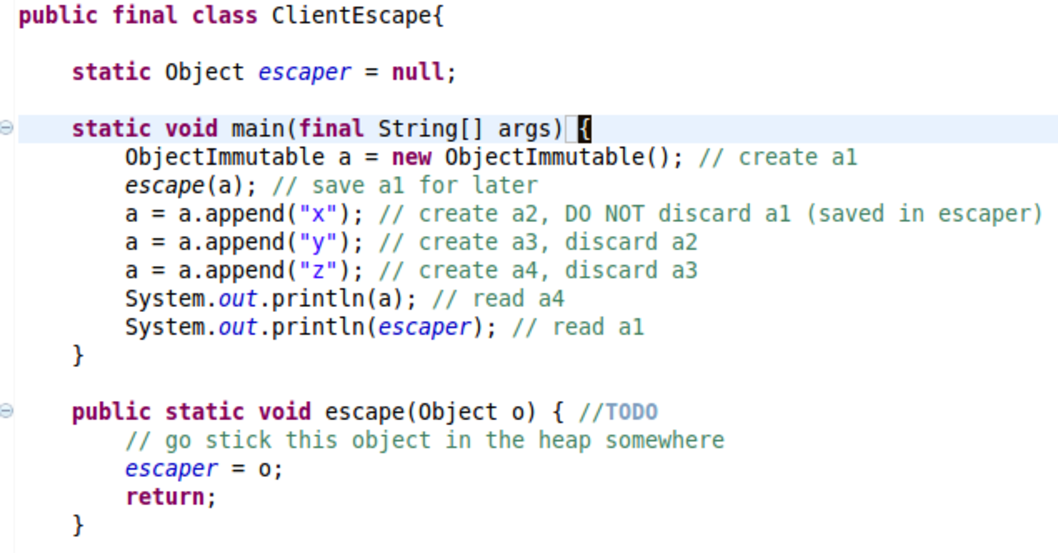
\includegraphics[width=0.5\textwidth]{img/client_escape}
\end{figure}

Figure \ref{fig:client_escape} presents an example of a client where an object is escaping the stacking and is creating a pointer to the heap. The points to note here is that at the second line of the method, the instantiated Immutable object is being passed as a parameter to a method. Inside the \texttt{escape()} method, the immutable object is assigned to a static global variable. Since global variable can be accessed in multiple methods, this causes the immutable object to have a reference to the heap which causes it to be globally accessible. This is a case when an object is said to have ``escaped''. In the main method again, it can be noticed that at the end of the method, the assigned static global variable \texttt{escaper} is being used, which stores the same reference in the heap as the first instance of the local variable \texttt{a}. Now, since the local object was immutable in nature, the heap reference stores the original instance, and when the global variable is referenced at a subsequent program point it successfully returns the original instance of the object. However, if the local object was mutable instead, it would lose its original instance through the mutator methods between the program point where  the object is escaping and when the escaped object is being referenced at a later program point. So an erroneous value for the local object would be returned. The objective of this analysis is to detect this use cases through escape analysis and detect which objects in a method can be transformed to mutable.
%Its Safe to mutate client
%What it is safe to convert t
%The Case where it cannot be transformed
%Explain object escaping
\section{Overview of analysis}\label{sec:analysis}
%Mention the two steps. Dataflow analysis step. and then the escape analysis step.
%Insert a pseudocode snippet
For the scope of ECE750, only the intra-procedural analysis of the complete program analysis is completed. This mean that, for this project, the functionality of the program is only limited to doing intra-procedural analysis on a given method to detect whether an immutable local variable or a field reference escapes at a certain program point in a method, and checks whether a variable with the same \textit{Object Representative} is used at a later program point. If such a case does happen, then because of the use case of the immutable object in the respective method, the object cannot be transformed to mutable. Firstly, this section explains the intra procedural dataflow analysis that happens in the program. Secondly, it explains the reason for the usage of Object Representatives \cite{ref:or} in the scope of the data flow analysis. Lastly the escape analysis rules used in the project to detect object escaping is explained. The intra-procedural analysis is done using the dataflow analysis API provided by the Soot framework \citep{ref:Soot}.

\subsection{Dataflow Analysis}\label{sec:dataflow}
The dataflow analysis is a ``may-alias'' forward analysis, where each unit in the analysis graph stores a HashMap of the local variables or field references and their object representatives at the respective program point. Each of the design choices for the data flow analysis are explained below.

\textbf{Direction of Analysis:} The direction of the analysis is chosen to be forward analysis because in each step of the flow through function, the information about the variables in previous program points is of interest to subsequent program points. This is important because in the escape analysis step of the algorithm followed by the dataflow analysis step, the object representatives mapping of the variable from previous program points is used to determine whether it is safe to make the object immutable or not.

%Flowthrough with Object Representative
\textbf{Flowthrough Reaching Condition:} The reaching condition for the flowthrough of information in a unit done according to the following rules. Each unit of the analysis graph stores a HashMap that stores an instance of the Local variable of a field reference along with its Object Representative that is generated along the flowthrough function.
\vspace{5mm}

\begin{algorithm}
\caption{Flowthrough algorithm for dataflow analysis}
\label{fig:flowthrough}
\begin{algorithmic}
  \State Copy InSet to OutSet\;
  \If{Stmt is DefinitionStmt}
	\If{rhs is LocalVariable}
		\State OutSet.put(lhs, rhs.ObjectRep)\;
	\Else
		\State generateObjectRep\;
		\State OutSet.put(lhs, newObjectRep)\;
	\EndIf	

  \EndIf
\end{algorithmic}
\end{algorithm}
%Mayalias(merge)
\textbf{Merge Condition: } The merge condition for this analysis is done in the form of May-Analysis, because a variable may attain different ObjectRepresentatives in different branches. In that case, both the object representative for the object are stored with respect to the program point in which the merge is happening. This is necessary because if the object escapes within the branch, and in a subsequent program pointer if either of the Object Representatives aliases with a variable being used in the Stmt, then the object is still considered to be non-transformable to mutable because the used object ``may'' have escaped in a branch. This is a may-analysis because information about both the branches are recorded for analysis rather a definitive must analysis where the same condition must hold for both branches.

\subsection{Object Representatives}\label{sec:OR}
%Talk about what is object representative (Cite)
In this analysis Object Representatives need to be used because in this analysis objects aliasing with respect to their pointers to the heap are of interest rather than their value assignments in the stack. Generally in order to infer object reference to the heap, an inter-procedural analysis is necessary. However object representatives are a technique of dereferencing heap pointers to local objects from within an intra-procedural analysis \cite{ref:or}.

This is evident in our analysis of the client with the escaping object shown previously in figure \ref{fig:client_escape}. In that example, the escaped instance of \texttt{a} would have the same object representative as the field \texttt{escaper}, that is called later in the program although they were assigned to the heap in a seperate method from the subject method. If instead, an integer value assignment for the object instance and the field was used during the dataflow analysis, then this analysis would not be possible because they would have different value assignments. Without dereferencing pointers to the heap there is no way for programs to do this aliasing without using object representatives.
%Talk about why object representative is needed.
%How it is applied in this regard

\subsection{EscapeAnalysis}\label{sec:escape}
%Introduce the concept from the paper (cite)
In this program, escape analysis is used to detect objects that are escaping the stack to the heap, which causes objects to be globally accessible and hence prevent tranformation. There has been much work centered around escape analysis in the last decade, most of which has been towards its application in creating thread safe programs and optimizing multithreaded programming. The papers by Choi et al. and Vivien et. al \cite{ref:escapejava}\cite{ref:incrementalescape} were some of the first papers to introduce the escape analysis in the context of inter-procedural analysis. Both the papers were focused on the application of escape analysis to minimize object allocation to the heap with the objective of reducing sychronization operation for threads.

Surprisingly, escape analysis is seldom used in the context of intraprocedural analysis. The only work that relates to this project with respect to escape analysis is its application in dynamic compilation and deoptimization \cite{ref:globalescape} which uses escape analysis both in the context of intraprocedural analysis interprocedural analysis. Much of the intraprocedural inference techniques used in this work has been inspired by the works presented there.

%Talk about the rules with respect to this analysis (one paragraph each)
There are many programming use cases which causes local objects inside methods to escape the stack and get allocated to the heap, however in the scope of this research only some rules apply to the analysis. The applicable rules of escape analysis that apply in this context are strictly those related to object instance sharing and accessibility. According to existing research \cite{ref:globalescape} there are two categories of object escaping: \textit{global escape} \& \textit{method escape}. In the context of this research only the global escape of objects is relevant. Objects that suffer from method escape are also called \textit{thread-local} objects which means that the object has escaped the context of the method, but is local with respect to the thread running the method. Since the focus of this analysis is not to optimize synchronization calls with respect to threading, this type of object escape not relavant for this analysis.

The cases of \textit{global escape} relevant to this research is listed below:

\texttt{T.sf = a :} A local variable escapes its local allocation on the stack to the heap when it is assigned to a static field of the class. Being assigned to the static field of a class allows the object instance to be referenced by multiple methods and that is causes the object to escape. In terms of static analysis, this can checked trivially by checking that the left operand is a member of the field deference list, and that it of type \texttt{static}, then checking that the right operand is a local variable, in which case the assignee is the variable escaping ie.\ \texttt{a}.

\texttt{p.f = a :} When local variable is assigned to the field of another local variable, the assigned local variable is defined as escaped. The reason for this is that, if the assignee is mutable, and it is assigned to field of another local variable, any changes to the field of the local variable will cause the assigned variable to be changed as well. This is shown in the sample code segment in figure \ref{fig:fieldassignment}.

\begin{figure}[H]
	\caption{Object escape with local field assignment} \label{fig:fieldassignment}
	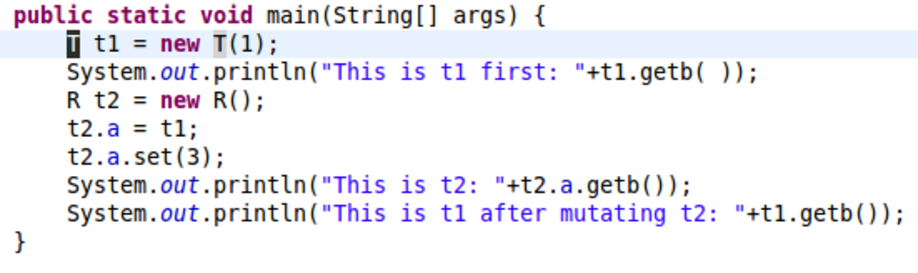
\includegraphics[width=0.5\textwidth]{img/fieldassignmentcod}
	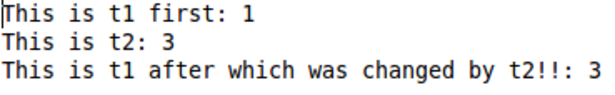
\includegraphics[width=0.3\textwidth]{img/fieldassignmentresult}
\end{figure}

In figure \ref{fig:fieldassignment} two local variable objects \texttt{t1} and \texttt{t2} are created, where \texttt{t2} owns an attribute with the same type as \texttt{t1} where \texttt{t1} is mutable. \texttt{t1} is assigned to the field \texttt{a} of t2 and followed by that the field of \texttt{t2} is mutated. After the mutation, it is seen from the output that due to the change in the field of \texttt{t2} the original variable also gets changed. It is difficult to resolve this aliasing in the dataflow analysis because the dataflow analysis only stores the object representatives of the local variables, but it does not store the object representatives of the fields of the local variables. Therefore, it is conservatively assumed in this analysis that whenever a local is assigned to the field of another variable, the assignee is marked as ``escaped'' irrespective of whether the field of the local variable actually gets mutated or not. This could have been avoided if the implementation of the type of \texttt{t1} was immutable, so that the \texttt{set()} method of object returned a new instance of the object, rather mutating the existing attribute.
%put an algorithm snippet if possible

\texttt{foo(a) :} A local variable is declared as escaped when it is passed as a parameter to another method. The reason for this is that the calling method could possibly mutate the object. From just intra procedural analysis it is impossible to know whether the calling method will actually mutate the object or not, and therefore for this analysis it is conservatively assumed that when an object is passed as a parameter to another method it has escaped the stack and is therefore deemed as escaped. Ideally it would be possible to check the operations on the passed in variable through an interprocedural analysis where one can transitively analyze whether any of the pointers of the object are being mutated by the calling methods. However, the inter-procedure analysis is beyond the scope of this project and is therefore a possible candidate for future work. This case of \textit{global escape} is being exhibitted in figure \ref{fig:client_escape} in section \ref{sec:example}. In that example, the local variable was being passed as a parameter to the method \texttt{escape()} and therefore at that program point that specific instace of the variable \texttt{a} is flagged as ``escaped''.


\section{Implementation and Evaluation}
%Describe the overall algorithmmen
The implementation of the analysis was completely done with the Soot framework\citep{ref:Soot} for Java bytecode analysis. Below in figure \ref{fig:overall} the wrapper algorithm that uses the escaped analysis and the result of the dataflow analysis is presented.

\begin{algorithm}
\caption{Wrapper algorithm for detect mutable safety}
\label{fig:overall}
\begin{algorithmic}
  \State Do dataflow analysis\;
  \For{Each node \texttt{n} in the dataflow graph}
       \State rhs = Value for Stmt.rhs
       \If{rhs is escaping in n}
           \State flag rhs as ``escaped''
       \EndIf
       \State rhsObjRep = Object Representative for rhs
       \If{rhsObjRep equals Object Representative for existing local in the Map}
		  \If{Any of the aliasing locals are flagged as escaped}
		      \State Add the aliasing tuple to a flagged list
       	  \EndIf
       \EndIf
  \EndFor
  \State Filter the locals from the tuple set
  \State Flag the locals as unsafe to transform
\end{algorithmic}
\end{algorithm}

The analysis below returns a list of tuples from the intra-procedure and escape analysis of a method. The each tuple in the list indicate a set of local variables that have the same object representative pointer to the heap, with atleast one of them escaping and being read by the method at a subsequent program point. The tuples contain not just the locals and fields of the method but also many temporary variables that are introduced by Soot's intermediate form for bytecode analysis. Therefore all the temporary variables are filtered from the tuples sets, and all the Locals from the tuple set are stored in a separate list and this elements of this list indicate which varaibles in this method are unsafe to be transformed to mutable from their immutable declaration.

%Talk about the results of the analysis. %Talk about the limitations of the analysis
The result of the analysis by soot returns a list of variables for each method of the analyzed class that are unsafe to be transformed to mutable. In the bigger scheme of things, what we really interested in is which variables are not in that list because we care more about the variables that can be transformed. For now the analysis has only been tested on toy test cases created during the development of the analysis technique and it has not been run on widely used Java library classes. The limitations of this analysis is that it only addresses the core analysis behind detecting when it is safe to transform immutable object using escape analysis. However for the analysis to be useful, it first needs to infer which objects are immutable to begin with, because we don't care about the variables that are already mutable. Existing research, for example the work of C.Unkel et. al \cite{ref:finalinference} can be used to inference objects with immutable declarations. This would be used to further filter from the list of flagged variables that is returned by this analysis, because currently is returns the list of all variable in a method that are escaping and being read afterwards, whether they are mutable or immutable.

The current analysis returns correct results within the use case domain explored during the development of the analysis. However, the analysis must run on actual useful code in order to validate its utilty.
\section{Future Work}
%I want it to do interprocedural with call graph.
Currently the analysis is strictly intra-procedural and returns the variables that are unsafe to transform within the scope of the methods inside the class. However, for the analysis to be scalable a inter-procedural analysis needs to take place prior to the intra-procedural analysis to generate a call graph for a certain object that is of interest, and then analyze the methods that define the call sites using the analysis defined in this project. This way, the user can test specific immutable objects whether it is safe to transform them to mutable and the interprocedural analysis will transitively analyse the calling methods of the object to make the inference.

%It needs to do program transformation for call sites and the object mutator and constructor
After the inference is made whether an object can be made mutable or not, certain program transformation needs to take place to make this change happen. Broadly are two abstraction in which the transformations will take place. One of them is the object itself, where the object attribute declarations need to be changed to mutable rather than immutable. Also in object, the mutator methods need to be change mutate the instance itself rather than returning a new instance of the object. The abstraction where the transformation needs to take place are the call sites of the respective object. The call site need to be transformed to reflect the changes that have been made to the object as a result of the analysis. For this to happen certain formal transformation rules need to be defined, and this in itself would have its own program analysis.

%Metrics to compare.
After the interprocedural analysis and the transformation rules are finalized, the program analysis will finally be ready testing on production level code. In order to instrument the contribution and utility of this analysis there are two metrics that would be interesting to consider after it has been run through benchmark programs:
\begin{enumerate}
\item Finding what percentage of immutable object declarations actually qualify as ``safe to transform'' according to this analysis
\item After the transformation, what is the performance and memory usage improvement for the subject programs.
\end{enumerate}
\section{Conclusion}
Talk about the projects impact, result of evaluations and experience.
%Possible contributions
%Experience


% For peer review papers, you can put extra information on the cover
% page as needed:
% \ifCLASSOPTIONpeerreview
% \begin{center} \bfseries EDICS Category: 3-BBND \end{center}
% \fi
%
% For peerreview papers, this IEEEtran command inserts a page break and
% creates the second title. It will be ignored for other modes.
\IEEEpeerreviewmaketitle





% trigger a \newpage just before the given reference
% number - used to balance the columns on the last page
% adjust value as needed - may need to be readjusted if
% the document is modified later
%\IEEEtriggeratref{8}
% The "triggered" command can be changed if desired:
%\IEEEtriggercmd{\enlargethispage{-5in}}

% references section

% can use a bibliography generated by BibTeX as a .bbl file
% BibTeX documentation can be easily obtained at:
% http://www.ctan.org/tex-archive/biblio/bibtex/contrib/doc/
% The IEEEtran BibTeX style support page is at:
% http://www.michaelshell.org/tex/ieeetran/bibtex/
\bibliographystyle{IEEEtran}
\bibliography{bib/report750}
% argument is your BibTeX string definitions and bibliography database(s)
%\bibliography{}


%
% <OR> manually copy in the resultant .bbl file
% set second argument of \begin to the number of references
% (used to reserve space for the reference number labels box)



% that's all folks
\end{document}


